% PRESAGE teaser / system overview. Self-contained TikZ (no fontawesome).
\begin{figure*}[t]
\centering
\resizebox{\textwidth}{!}{%
\begin{tikzpicture}[
  font=\small,
  stage/.style={draw, rounded corners=3pt, align=center, inner sep=4pt, minimum height=1.0cm, font=\footnotesize},
  detail/.style={font=\scriptsize\itshape, text=black!60, align=center},
  arr/.style={-{Stealth[length=2.4mm]}, thick, black!65},
  grouplabel/.style={font=\small\bfseries\sffamily},
]

% ================= TOP TIER: KNOWLEDGE CURATION =================
\node[stage, fill=green!8, minimum width=2.0cm] (web) {Extension\\\textbf{web sources}\\[-1pt]{\tiny CPN, university}};
\node[stage, right=0.7cm of web, fill=green!14, minimum width=2.2cm] (canon) {\textbf{Canonical KB}\\[-1pt]{\tiny cited symptom text}\\[-1pt]{\tiny 335 crops / 1{,}251 dis.}};
\node[stage, right=0.9cm of canon, fill=orange!8, minimum width=2.3cm] (imgs) {state-stratified\\\textbf{field images}\\[-1pt]{\tiny Bugwood, geo-tagged}};
\node[stage, right=0.7cm of imgs, fill=orange!14, minimum width=2.2cm] (vlm) {per-image\\\textbf{VLM delta}\\[-1pt]{\tiny canonical $\!\to\!$ image\_shows}};
\node[stage, right=0.7cm of vlm, fill=orange!20, minimum width=2.1cm, thick] (delta) {\textbf{Delta KB}\\[-1pt]{\tiny per (disease, state)}\\[-1pt]{\tiny image-grounded}};

\draw[arr] (web) -- (canon);
\draw[arr] (imgs) -- (vlm);
\draw[arr] (vlm) -- (delta);
\draw[arr, densely dashed, black!45] (canon.south) to[out=-60,in=120] (vlm.north)
  node[midway, font=\tiny, text=black!55, fill=white, inner sep=1pt] {grounds};

% ================= BOTTOM TIER: COST-EFFECTIVE INFERENCE =================
\node[stage, below=2.4cm of web.west, anchor=west, fill=black!4, minimum width=1.5cm] (test)
  {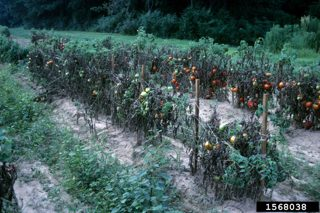
\includegraphics[width=0.9cm,height=0.9cm]{figures/delta_early_blight.jpg}\\[1pt]{\tiny test image}};
\node[stage, right=0.7cm of test, fill=blue!8, minimum width=2.2cm] (enc) {\textbf{frozen encoder}\\[-1pt]{\tiny BioCLIP, projector-tuned}\\[-1pt]{\tiny \emph{does all the looking}}};
\node[stage, right=0.7cm of enc, fill=blue!14, minimum width=2.3cm] (proto) {\textbf{image-prototype}\\\textbf{short-list} (top-5)\\[-1pt]{\tiny recall@5 $\approx$ ceiling}};
\node[stage, right=0.7cm of proto, fill=blue!14, minimum width=2.3cm] (ret) {\textbf{adaptive retrieval}\\[-1pt]{\tiny $k$ nearest cases}\\[-1pt]{\tiny label$+$sim \emph{as text}}};
\node[stage, right=0.7cm of ret, fill=purple!10, minimum width=2.4cm, thick] (llm) {\textbf{text-only LLM}\\[-1pt]{\tiny re-ranks short-list}\\[-1pt]{\tiny \textbf{never sees a pixel}}};
\node[stage, right=0.6cm of llm, fill=green!18, minimum width=1.7cm, thick] (pred) {\textbf{Prediction}\\[-1pt]{\tiny\itshape Early Blight}};

\draw[arr] (test) -- (enc);
\draw[arr] (enc) -- (proto);
\draw[arr] (proto) -- (ret);
\draw[arr] (ret) -- (llm);
\draw[arr] (llm) -- (pred);
% Delta KB feeds symptom evidence into the LLM
\draw[arr, densely dashed, orange!70!black] (delta.south) to[out=-90,in=90] (llm.north)
  node[midway, font=\tiny, text=orange!60!black, fill=white, inner sep=1pt] {\,symptom evidence\,};

% cost badge
\node[draw=green!45!black, rounded corners=3pt, fill=green!6, font=\scriptsize, below=0.25cm of ret, align=center, inner sep=3pt] (cost)
  {\textbf{\$5} full sweep \quad vs.\quad \textbf{\$18--35}/crop image-streaming agent};

% ================= group boxes =================
\begin{scope}[on background layer]
  \node[draw=green!25, fill=green!2, rounded corners=8pt, inner sep=10pt,
        fit=(web)(canon)(imgs)(vlm)(delta)] (top) {};
  \node[grouplabel, anchor=north west, text=green!40!black] at ($(top.north west)+(0.12,-0.04)$) {Knowledge Curation};
  \node[draw=blue!22, fill=blue!3, rounded corners=8pt, inner sep=10pt,
        fit=(test)(enc)(proto)(ret)(llm)(pred)(cost)] (bot) {};
  \node[grouplabel, anchor=north west, text=blue!45!black] at ($(bot.north west)+(0.12,-0.04)$) {Cost-Effective Retrieval--Reasoning Inference};
\end{scope}

\end{tikzpicture}
}%
\caption{\textbf{\textsc{Presage} overview.} \emph{Top (Knowledge Curation):}
cited canonical symptom text is mined from extension sources, then
\emph{grounded} per (disease, state) by a VLM that captions state-stratified
Bugwood field photographs, yielding an image-grounded \textbf{Delta KB}.
\emph{Bottom (Inference):} we factor perception from reasoning---a frozen
domain encoder produces an image-prototype short-list (with near-ceiling
recall@5) and an \emph{adaptive} similarity-retrieved evidence set, and a
text-only language model re-ranks using that evidence plus Delta-KB symptoms.
The language model \textbf{never sees a pixel}, collapsing per-crop cost from
\$18--35 (image-streaming agents) to a few dollars for the entire sweep.}
\label{fig:teaser}
\end{figure*}
